\documentclass[11pt,a4paper]{article}

\usepackage[utf8]{inputenc}
\usepackage[T1]{fontenc}
\usepackage[english]{babel}
\usepackage{lmodern}
\usepackage{amsmath,amssymb,mathtools}
\usepackage{mathrsfs}
\usepackage{graphicx}
\usepackage{float}
\usepackage{caption}
\usepackage{geometry}
\usepackage{hyperref}

\geometry{margin=2.25cm}
\graphicspath{{figures_compressed/}}
\setlength{\parindent}{0pt}
\setlength{\parskip}{0.55em}
\captionsetup{font=small}
\hypersetup{
  colorlinks=true,
  linkcolor=black,
  urlcolor=black,
  pdftitle={Sprites -- Physics I, PC Section, CCMP 2023},
  pdfauthor={Concours Commun Mines-Ponts}
}

\newcommand{\question}[1]{%
  \par\medskip\noindent\textbf{\(\square\)\ #1.}\quad%
}

\begin{document}

\begin{center}
{\small Concours Commun Mines-Ponts (CCMP) -- 2023 Session\\
PC Section -- Exam: Physics I}

\vspace{0.6em}
{\Large\bfseries Sprites}
\end{center}

A formula sheet and numerical data are provided at the end of the problem statement.
All numerical estimates should be carried out to one significant figure.

Sprites are very intense, relatively brief red luminous emissions, lasting on the order of a few hundred milliseconds, which occur between cloud tops and the ionosphere. Most of them are located between 40 and 80~km in altitude. They have only been observed and studied since about 1990. Some of their manifestations had already been reported much earlier, but observing them from the ground is difficult. Sprites are part of a group of luminous emissions that occur during thunderstorms. The same group also includes blue jets and elves; see Figure~\ref{fig:formes}. These emissions are the consequence of large electric currents produced during an avalanche-like production of ions and electrons. The avalanche may be initiated by a cosmic-ray particle. During collisions with molecules, the electrons in the electric currents transfer energy to the molecules, which is subsequently lost through the emission of visible light.

\begin{figure}[H]
\centering
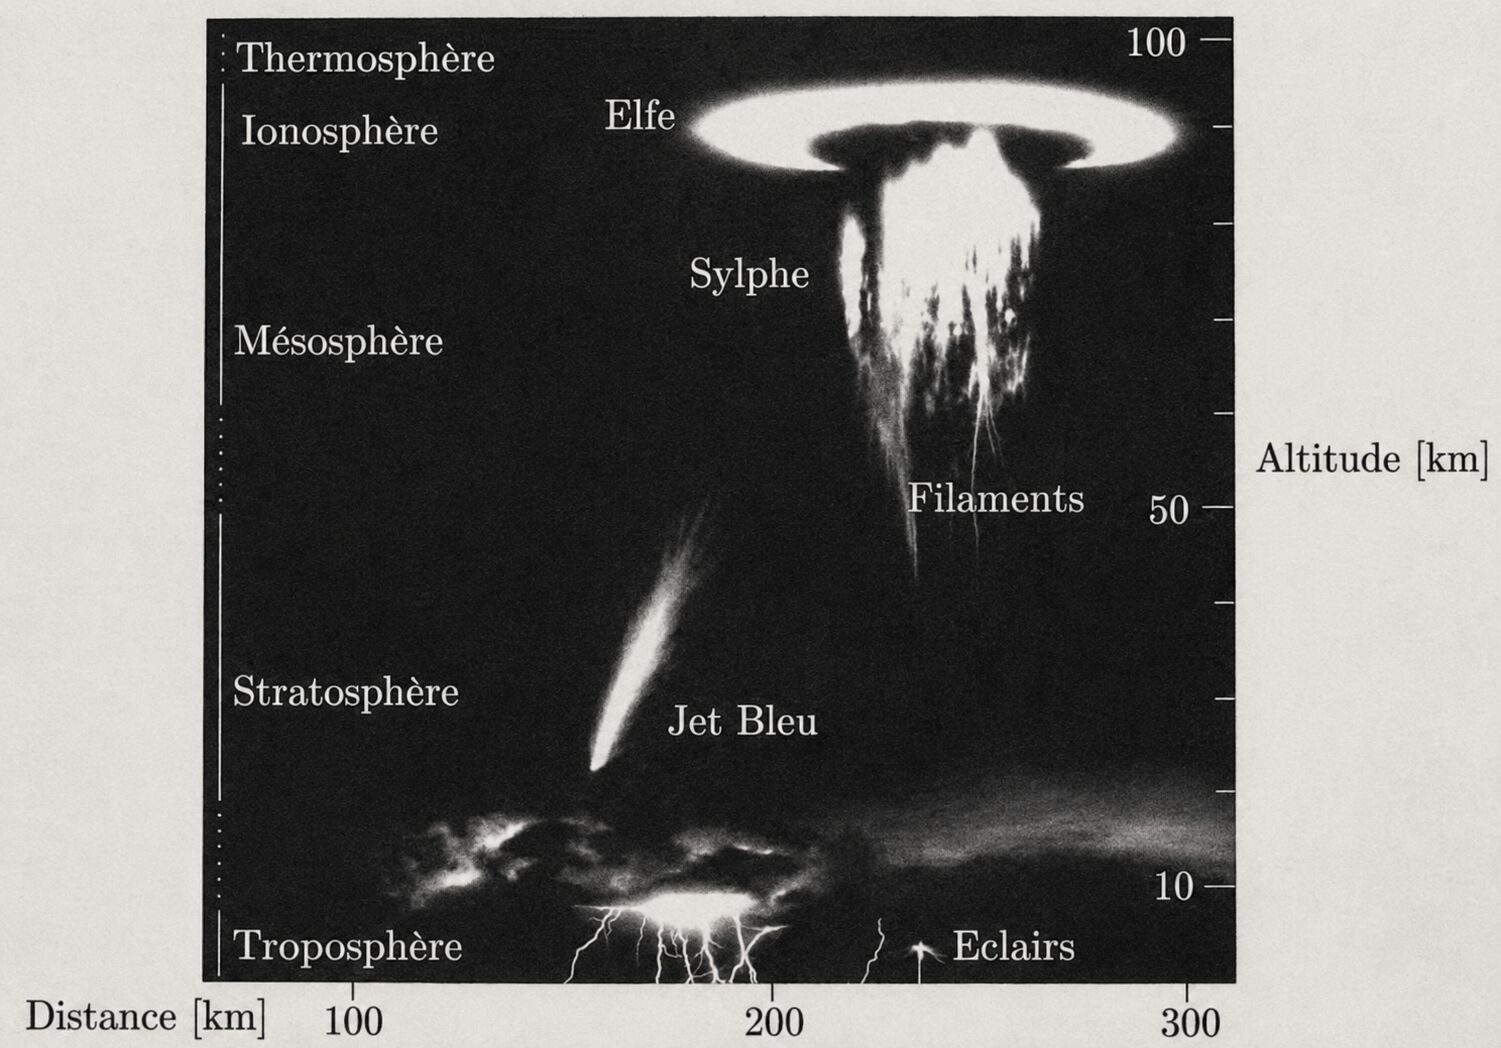
\includegraphics[width=0.78\linewidth]{figure_01.jpg}
\caption{Different types of atmospheric transient luminous events.}
\label{fig:formes}
\end{figure}

This problem contains three largely independent parts. The first concerns the observation of sprites. The second studies electrical properties of the atmosphere. The final part presents the model of avalanche formation of the current that gives rise to sprites.

\section*{I. Observation of Sprites}

\question{1}
Using the curves in Figure~\ref{fig:spectre}, justify the characteristic color of sprites. Also justify why they are difficult to observe from the surface of the Earth.

Despite this difficulty, images of sprites have been obtained, such as those in Figure~\ref{fig:photos}, which were observed from the Pic du Midi de Bigorre Observatory. Sprites were seen there above the Alps. The Pic du Midi de Bigorre is located in the middle of the Pyrenees mountain range, which extends from Perpignan in the east to Biarritz in the west, separating France from Spain.

\begin{figure}[H]
\centering
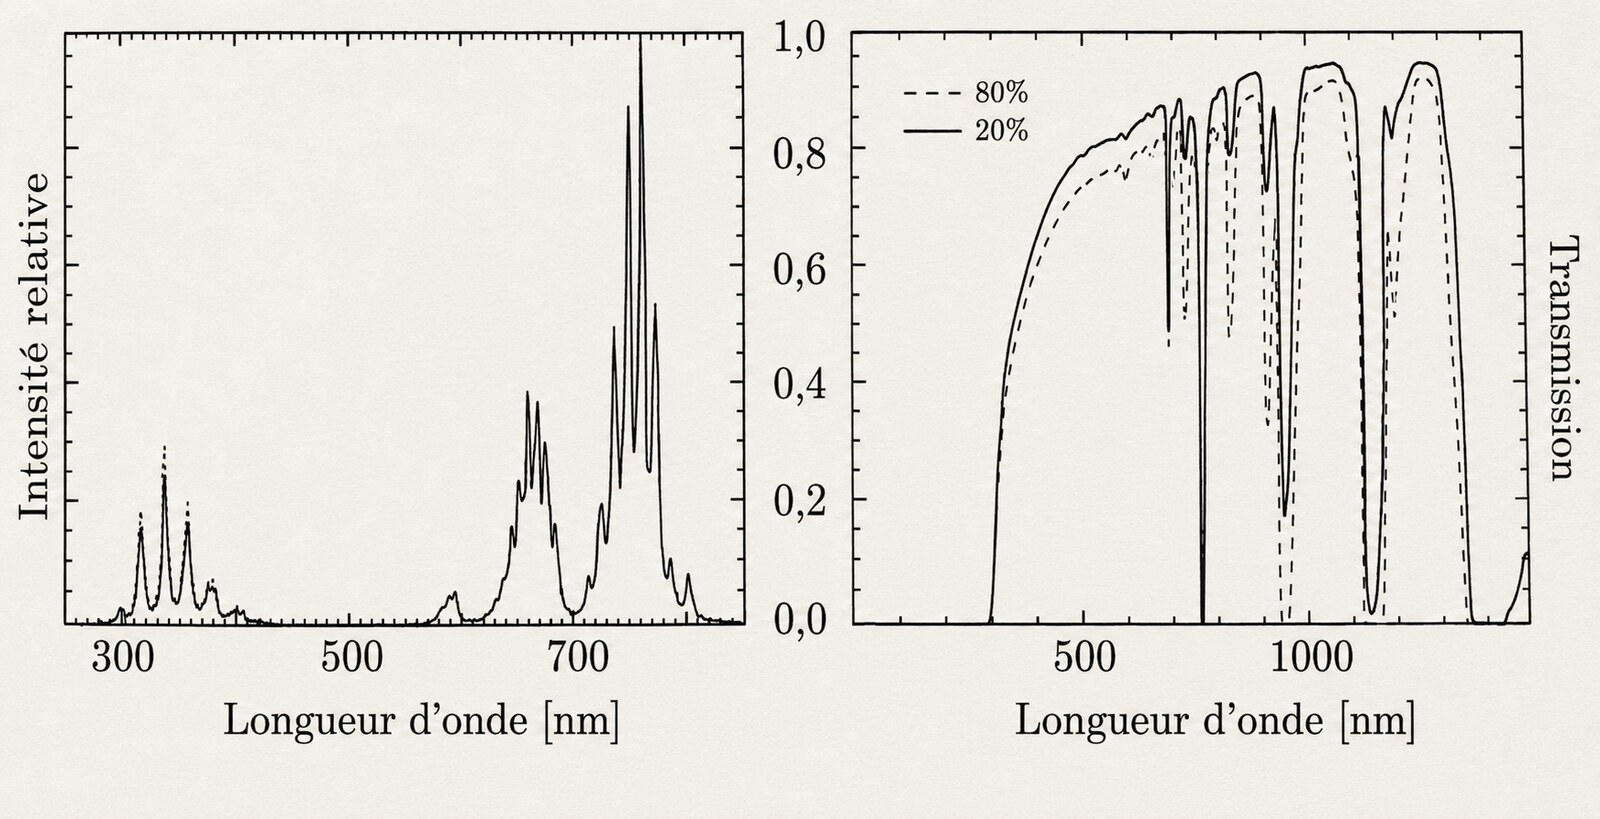
\includegraphics[width=0.88\linewidth]{figure_02.jpg}
\caption{Left: emission spectrum of a sprite. Right: atmospheric transmission coefficient for two humidity levels, 20~\% and 80~\%. These measurements were made by a ground-based detector placed below a source located at an altitude of 80~km. Figure taken from the article \textit{Spectrum of Red Sprites}, G.~Milikh, J.~A.~Valdivia and K.~Papadopoulos, \textit{Journal of Atmospheric and Solar-Terrestrial Physics}, vol.~60, pp.~907--915, 1998.}
\label{fig:spectre}
\end{figure}

Because of the curvature of the Earth, whose radius is \(R_T\), we consider whether it is possible to see sprites above the Alps.

\begin{figure}[H]
\centering
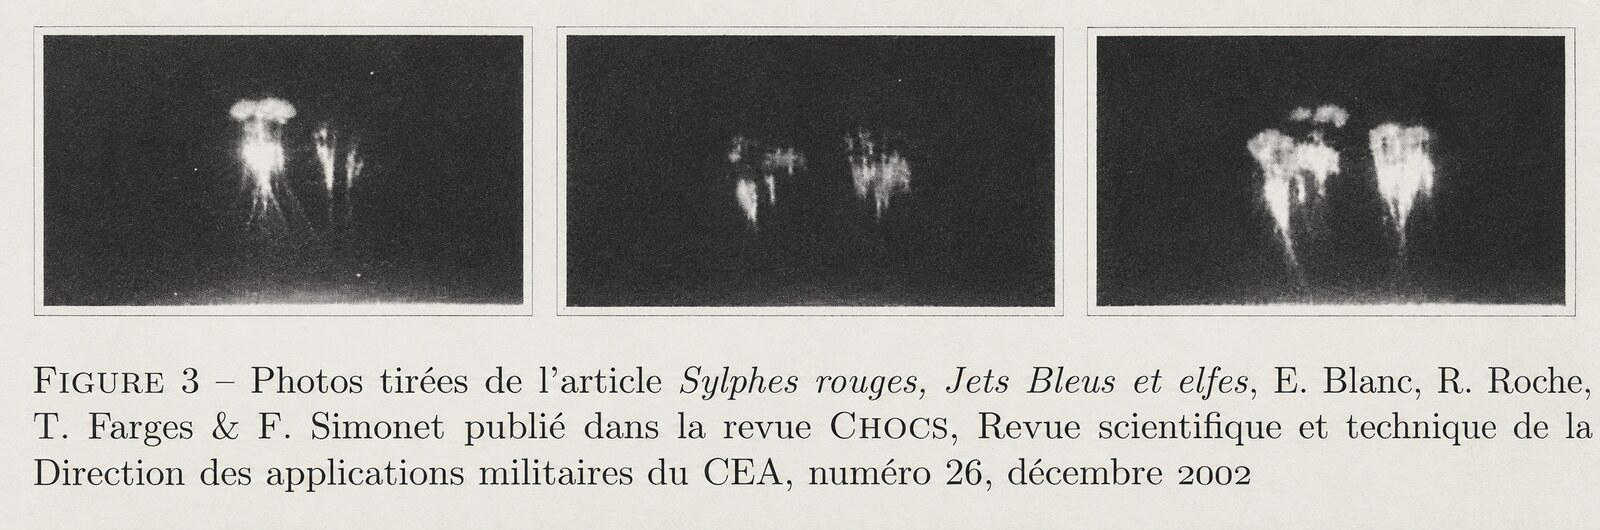
\includegraphics[width=0.88\linewidth]{figure_03.jpg}
\caption{Photographs taken from the article \textit{Sylphes rouges, jets bleus et elfes} [Red Sprites, Blue Jets and Elves], E.~Blanc, R.~Roche, T.~Farges and F.~Simonet, published in the journal \textsc{Chocs}, the scientific and technical journal of the CEA Directorate of Military Applications, issue~26, December~2002.}
\label{fig:photos}
\end{figure}

\question{2}
Is the straight-line distance \(d\) between the Pic du Midi de Bigorre and the French Alps on the order of 500, 1000 or 1500~km?

Neglecting the altitude of the Pic du Midi de Bigorre, draw an appropriate diagram of the horizon line starting from it and passing above the Alps at an altitude \(h\). Under suitable assumptions, express \(h\) as a function of \(R_T\) and \(d\), then calculate its numerical value.

Is it possible to see Alpine sprites from the Pic du Midi de Bigorre without any atmospheric refraction effect? Can Mont Blanc be seen in good weather?

In order to observe sprites regularly and to develop research aimed at better understanding their origin, two microcameras fixed to a window have been used on the International Space Station (ISS) since 2001. Both cameras look in the vertical direction. One of the two cameras operates in the visible range, while the other is fitted with a very narrow passband filter centered at 761~nm. Figure~\ref{fig:iss} shows the two images obtained during a recording. This recording was made during a major thunderstorm.

In these images, the luminous intensity obtained is expressed in LSB (\textit{least significant bit}, a camera-specific unit of measurement). A conventional lightning flash produces a level of 836~LSB on the camera operating in the visible range and gives 30~LSB on the filtered camera.

\begin{figure}[H]
\centering
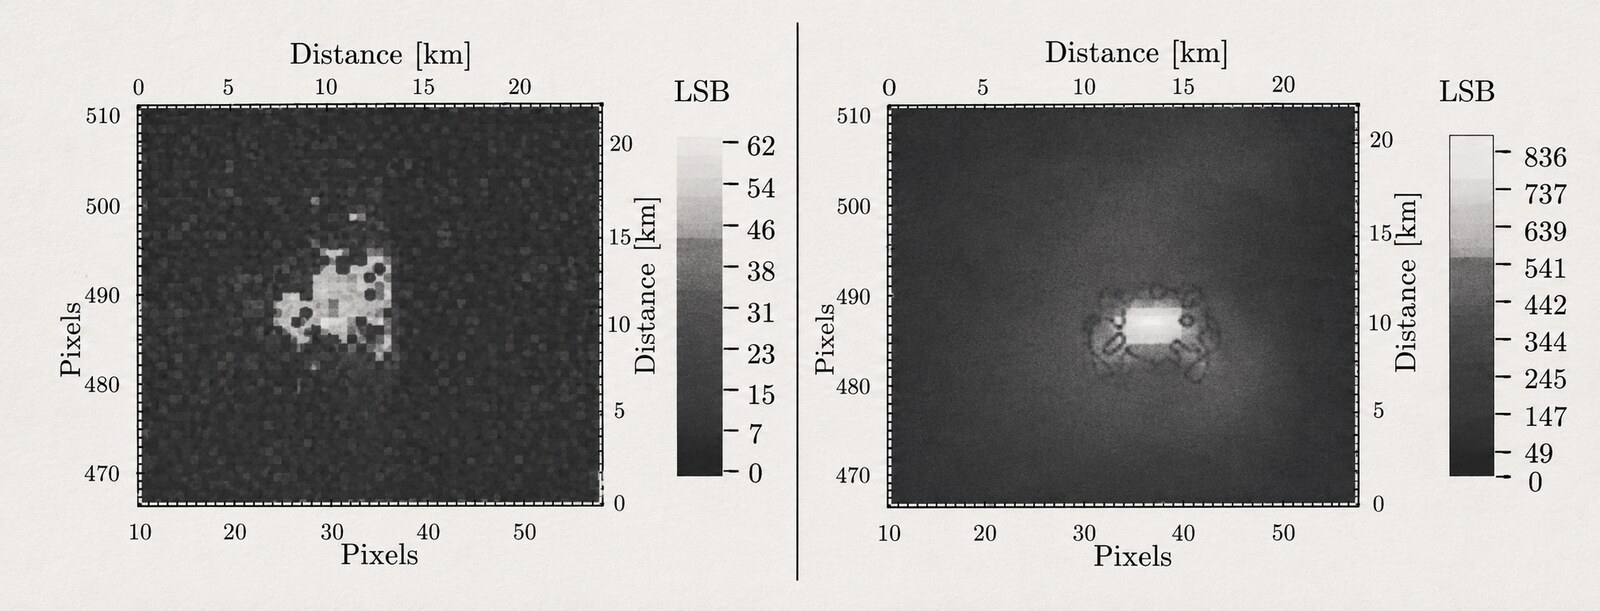
\includegraphics[width=0.86\linewidth]{figure_04.jpg}
\caption{Recordings made from the ISS by the filtered microcamera on the left and by the visible-range microcamera on the right. A black line isolates the detection of a sprite in the image on the right. Figures again taken from the article referenced in Figure~\ref{fig:photos}.}
\label{fig:iss}
\end{figure}

\question{3}
Show that analysis of the two images in Figure~\ref{fig:iss} does indeed prove the detection of a sprite.

\question{4}
The ISS is located at an altitude \(h_{\mathrm{ISS}}\) of about 400~km. Using Gauss's theorem and under certain assumptions that should be specified, show that the gravitational field it experiences is of the form
\begin{equation*}
G_{\mathrm{ISS}} = g_0 \left(1+\frac{h_{\mathrm{ISS}}}{R_T}\right)^{-2},
\end{equation*}
where \(g_0=9.8~\mathrm{m}\cdot\mathrm{s}^{-2}\) is the gravitational field at the Earth's surface.

\question{5}
After showing that it is constant, determine the expression \(v_{\mathrm{ISS}}\) for the magnitude of the velocity of the ISS in its circular orbit. Calculate its numerical value in \(\mathrm{km}\cdot\mathrm{s}^{-1}\).

\question{6}
Determine the expression for the revolution period \(T_{\mathrm{ISS}}\) of the ISS around the Earth and relate it to Kepler's third law.

\question{7}
The objective of the two ISS microcameras is to record the full evolution of a sprite during a pass above a thunderstorm. Comment on the feasibility and accuracy of these recordings. Justify your answers numerically.

It is difficult to observe sprites from the Earth in the visible range, because molecular oxygen \(\mathrm{O}_2\) in the atmosphere absorbs strongly at 762~nm. However, molecular oxygen becomes much rarer with altitude, allowing observations above an altitude of 40~km, as is the case with the ISS. We will study the evolution of the partial pressure \(P_{\mathrm{O}_2}(z)\) of molecular oxygen as a function of altitude \(z\). The model we use is the following:

\begin{itemize}
\item the atmosphere is treated as an ideal gas with molar mass \(M=29~\mathrm{g}\cdot\mathrm{mol}^{-1}\);
\item the mole fraction of molecular oxygen \(\mathrm{O}_2\) is assumed to be the same at every altitude \(z\) and equal to that at the Earth's surface, namely \(x_{\mathrm{O}_2}=20~\%\);
\item the atmosphere is assumed to be in equilibrium, so that the law of fluid statics applies; only weight, treated as the gravitational force, will be taken into account;
\item the pressure at the Earth's surface is \(P_0=1~\mathrm{bar}\) at \(z=0\), and the temperature is \(T_0=290~\mathrm{K}\);
\item the temperature evolves according to the law \(T(z)=T_0(1-z/\ell)\), with \(\ell=50~\mathrm{km}\), which necessarily restricts the model to altitudes below \(\ell\).
\end{itemize}

\question{8}
Recall, without proof, the vector form of the fluid-statics equation for a fluid of mass density \(\mu\).

Show that the atmospheric pressure \(P(z)\) satisfies the following differential equation:
\begin{equation*}
\frac{\mathrm{d}P}{\mathrm{d}z}
= -F(z)\frac{P}{H},
\qquad
F(z)=\frac{1}{(1-z/\ell)(1+z/R_T)^2},
\end{equation*}
where \(H\) is a characteristic length to be expressed in terms of \(R\), \(T_0\), \(M\) and \(g_0\). Evaluate \(H\) numerically in kilometers to one significant figure.

By decomposing the function \(F\), one may write
\begin{equation*}
F(z)=\frac{\alpha}{1-z/\ell}
+\frac{\beta+\gamma z}{(1+z/R_T)^2},
\end{equation*}
where the constants
\[
\alpha=\bigl[1+\epsilon(2+\epsilon)\bigr]^{-1},
\qquad
\beta=\alpha\epsilon(2+\epsilon),
\qquad
\gamma=\frac{\alpha\epsilon}{R_T},
\]
are introduced, provided that \(\epsilon=\ell/R_T\).

\question{9}
Show that, under the conditions of the problem, one may take \(\alpha\simeq 1\), \(\beta\simeq 2\epsilon\) and \(\gamma\simeq \epsilon/R_T\).

Show that the pressure \(P(z)\) in the atmosphere is then given by
\begin{equation}
P(z)=P_0
\left(\frac{1-z/\ell}{1+z/R_T}\right)^\xi
\exp\left[-\frac{z}{\chi(1+z/R_T)}\right],
\label{eq:pression}
\end{equation}
where the expressions for the quantities \(\xi\) and \(\chi\) in terms of \(\ell\), \(H\) and \(R_T\) should be specified.

\question{10}
What simplified expression for \(P(z)\) would you propose in light of the previous expression and of the values of the quantities involved in it? What approximation does this amount to making?

In Figure~\ref{fig:pression}, the pressure model of equation~\eqref{eq:pression}, with suitable parameter values, and the pressure measured by atmospheric and space probes are plotted on the same graph.

\begin{figure}[H]
\centering
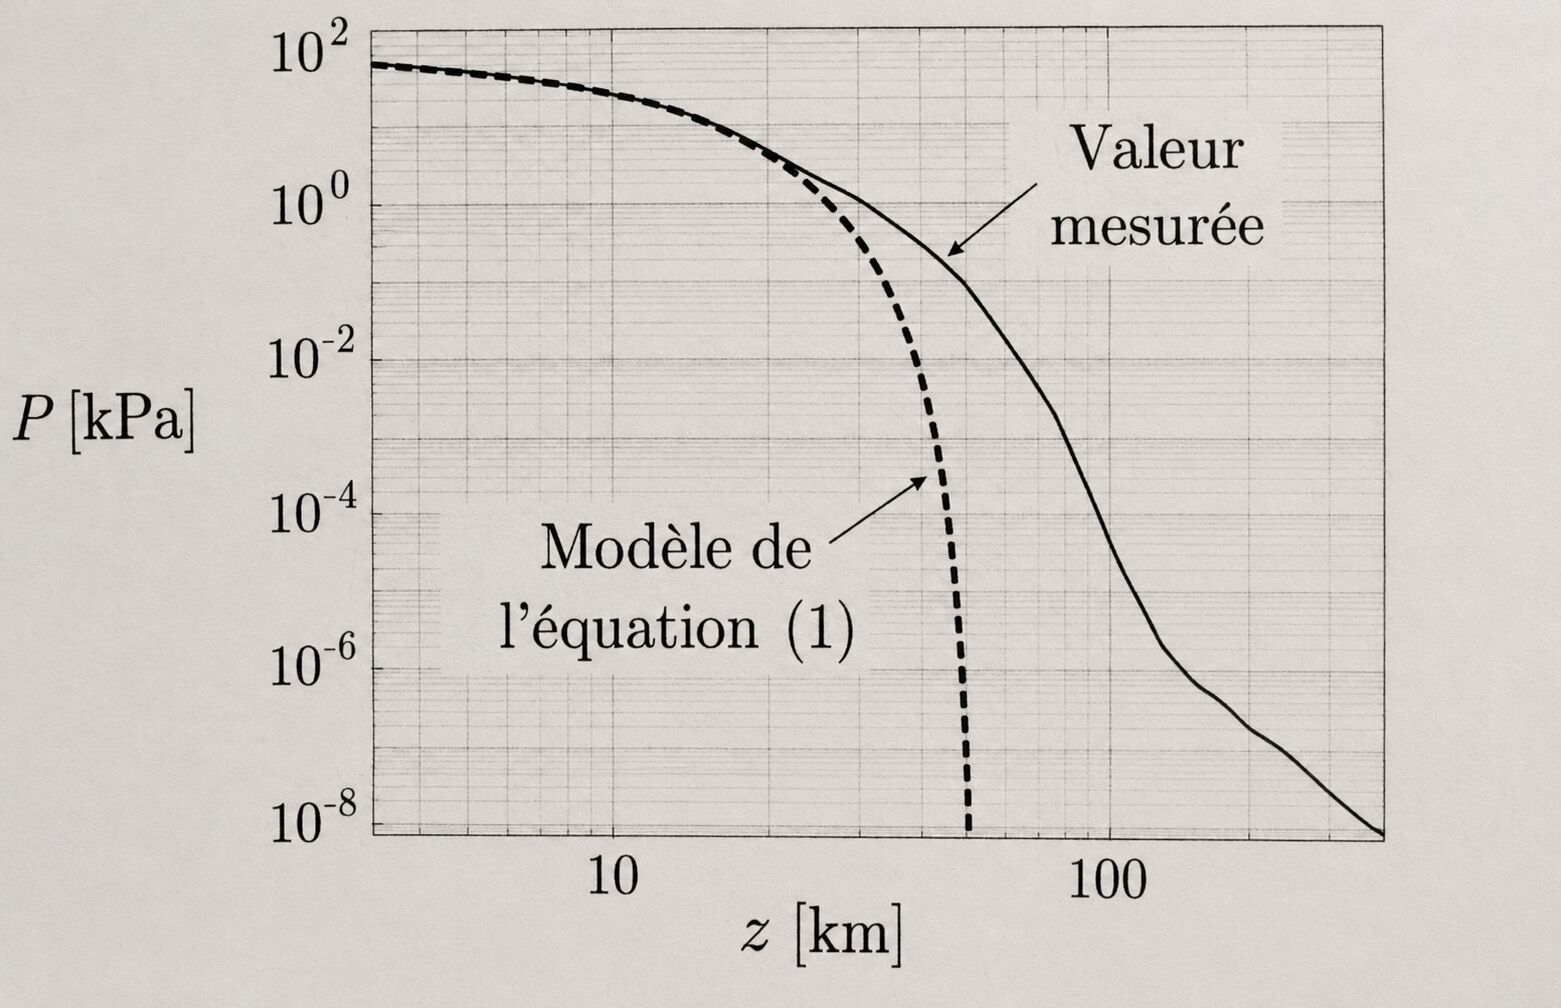
\includegraphics[width=0.72\linewidth]{figure_05.jpg}
\caption{Atmospheric air pressure.}
\label{fig:pression}
\end{figure}

\question{11}
What is the main reason why the model studied ceases to be valid from an altitude on the order of \(z=20~\mathrm{km}\), even though it is supposed to be potentially valid up to 50~km?

\question{12}
Discuss the possibility of observing sprites, in connection with the partial pressure of molecular oxygen, from the Earth and from the ISS.

\section*{II. An Electrical Atmosphere}

The atmosphere is treated as a plasma in which the electric current is mainly due to the motion of nonrelativistic electrons. The number density of mobile electrons is denoted by \(n\), the mass of an electron by \(m_e\), and its charge by \(e\).

First, we study the propagation of a monochromatic plane traveling electromagnetic wave with angular frequency \(\omega\), wave vector \(\vec{k}=k\vec{e}_z\), linearly polarized and described by its electric-field vector at time \(t\),
\[
\vec{E}=\vec{E}_0\exp\bigl(i(\omega t-kz)\bigr),
\qquad
\vec{E}_0\perp\vec{e}_z,
\qquad
\lVert\vec{e}_z\rVert=1.
\]

The atmosphere is characterized by the vacuum permittivity \(\varepsilon_0\) and the vacuum magnetic permeability \(\mu_0\). In this study, collisions undergone by the electrons and their weight are neglected. The only force acting on the electrons is the Lorentz force.

\question{13}
Show that the magnetic contribution to the Lorentz force on the electron is negligible compared with the electric contribution to that same force.

\question{14}
Justify why the contribution of the ions to the electric current is negligible compared with that of the electrons. Determine the relation between the complex representation of the electric field \(\vec{E}\) of the electromagnetic wave and that of the current density \(\vec{j}\) resulting from the interaction between the electron and \(\vec{E}\). Give the expression for the complex conductivity of the plasma \(\gamma_p\) and comment on this expression in terms of transferred power.

\question{15}
Establish the propagation equation for the electric field \(\vec{E}\). Deduce the dispersion relation satisfied by the wave vector \(k\).

\question{16}
What is the cutoff frequency \(f_p\), associated with a medium whose electron number density is \(n\), below which a wave sent from the Earth's surface can no longer propagate when it encounters that medium? Give the reasoning leading to this limit in detail. Carry out the numerical evaluation for a density \(n=10^{11}~\mathrm{m}^{-3}\), characteristic of sprites.

\question{17}
The image in Figure~\ref{fig:radar} shows the location and number of radar echoes returning to the transmitter. Analyze and comment on this map.

\begin{figure}[H]
\centering
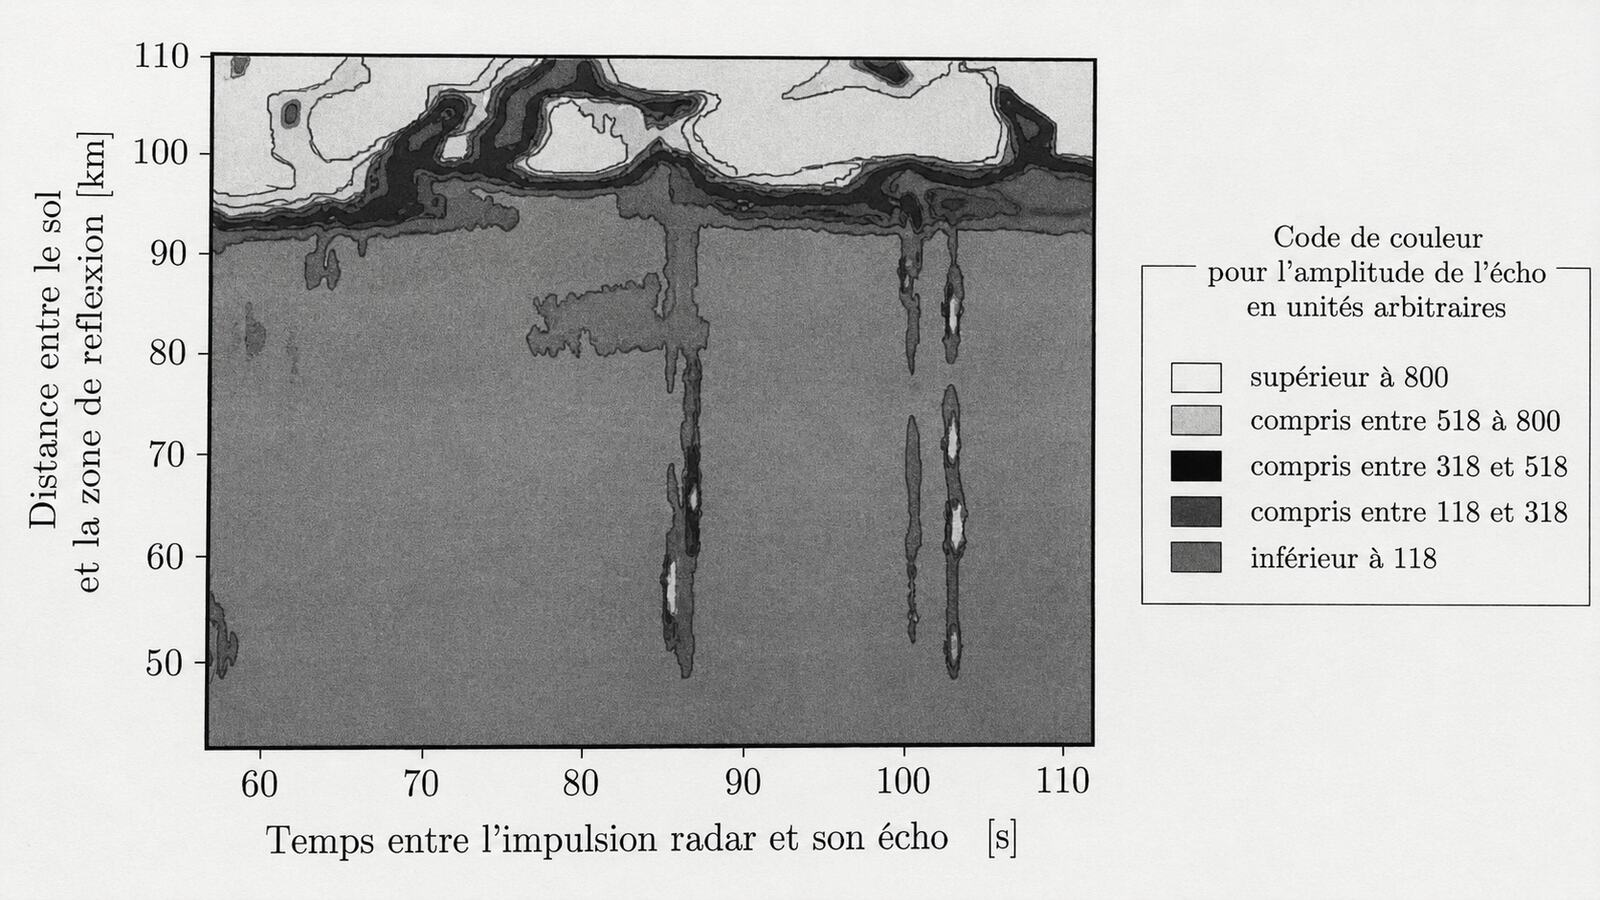
\includegraphics[width=0.86\linewidth]{figure_06.jpg}
\caption{Map of ground-based radar echoes at 2.2~MHz for the event recorded at 13:39 on 15 October 1994 at the Korhogo station (Côte d'Ivoire). Figure taken from the article \textit{HF echoes from ionization potentially produced by high-altitude discharges}, R.~A.~Roussel-Dupré and E.~Blanc, \textit{Journal of Geophysical Research}, vol.~102, no.~A3, pp.~4613--4622, 1997.}
\label{fig:radar}
\end{figure}

\section*{III. Avalanche Formation of a Current}

The origin of sprites is still being debated at present.
One model is based on the formation of a current linked to cascade ionizations caused by a primary electron capable of ionizing atmospheric molecules, mainly molecular nitrogen \(\mathrm{N}_2\), through successive collisions.
The secondary electrons created by the primary electron may in turn cause new ionizations, hence the avalanche effect. This primary electron may come from cosmic radiation, which constantly bathes the Earth. We will first study whether such an electron can ionize a molecular nitrogen molecule.

We consider a one-dimensional model along the axis \(Ox\), where \(N_0\) electrons move uniformly in the direction of increasing \(x\). These electrons are randomly distributed over a given cross-sectional area \(\Sigma\). Their motion takes place in a dilute medium where the molecular number density is \(n_{\mathrm{mo}}\). We are interested in the average distance \(\langle x\rangle\) they travel before undergoing a collision with a molecule. This distance is called the mean free path: \(\ell_{\mathrm{pm}}=\langle x\rangle\). Let \(N(x)<N_0\) be the number of electrons that have reached position \(x\) without undergoing any collision since \(x=0\). The probability that an electron undergoes a collision between positions \(x\) and \(x+\mathrm{d}x\) is the ratio of the total cross section associated with all the molecules present between \(x\) and \(x+\mathrm{d}x\) to the cross-sectional area \(\Sigma\). Each molecule is associated with an effective cross section \(S_{\mathrm{eff}}\), which represents the fact that if the electron reaches this area, a collision occurs, whereas if it passes beside it, no collision occurs.

\question{18}
By reasoning between \(x\) and \(x+\mathrm{d}x\), establish the differential equation governing the evolution of \(N(x)\). Solve this equation and express \(N(x)\) in terms of \(N_0\), \(n_{\mathrm{mo}}\), \(S_{\mathrm{eff}}\) and \(x\).

\question{19}
Show that the mean free path is
\[
\ell_{\mathrm{pm}}=\langle x\rangle=\frac{1}{n_{\mathrm{mo}}S_{\mathrm{eff}}}.
\]

\question{20}
For the molecular nitrogen molecule, \(S_{\mathrm{eff}}\simeq 10^{-20}~\mathrm{m}^2\). Justify this order of magnitude for the effective cross section. Determine the numerical value of the mean free path \(\ell_{\mathrm{pm}}\) for an electron at altitude \(z_3=60~\mathrm{km}\), where the pressure is \(P_3=20~\mathrm{Pa}\) and the temperature is \(T_3=260~\mathrm{K}\).

In the sprite region, there is an electric field whose main origin is, on the one hand, the charges present on cloud tops and, on the other, those present at the boundary between the mesosphere and the ionosphere, around 100~km altitude. Its magnitude is \(E\simeq 100~\mathrm{V}\cdot\mathrm{m}^{-1}\).

\question{21}
Given that the ionization energy of the molecular nitrogen molecule is \(\mathcal{E}_i\simeq 16~\mathrm{eV}\), can an electron initially at rest and accelerated by the local electric field of magnitude \(E\) ionize this molecule? Provide numerical arguments.

Relativistic cosmic electrons with a kinetic energy of 1~MeV are strongly suspected of initiating the avalanche cascade.

\question{22}
Justify why these cosmic electrons must necessarily be relativistic.

\question{23}
Explain the avalanche-cascade phenomenon.

We seek to determine when an average electron density \(n=10^{11}~\mathrm{m}^{-3}\), characteristic of sprites, is reached. Let \(\mathcal{N}\) denote the number of stages producing electrons during collisions. For simplicity, assume that all the electrons produced up to stage \(\mathcal{N}\) are contained in a volume whose characteristic length is \(\mathcal{N}\ell_{\mathrm{pm}}\).

\question{24}
Determine the numerical value of \(\mathcal{N}\). For this question, take the mean free path \(\ell_{\mathrm{pm}}\) to be on the order of one centimeter. You may use the curves in Figure~\ref{fig:fonctions}, explaining the procedure followed in detail.

\begin{figure}[H]
\centering
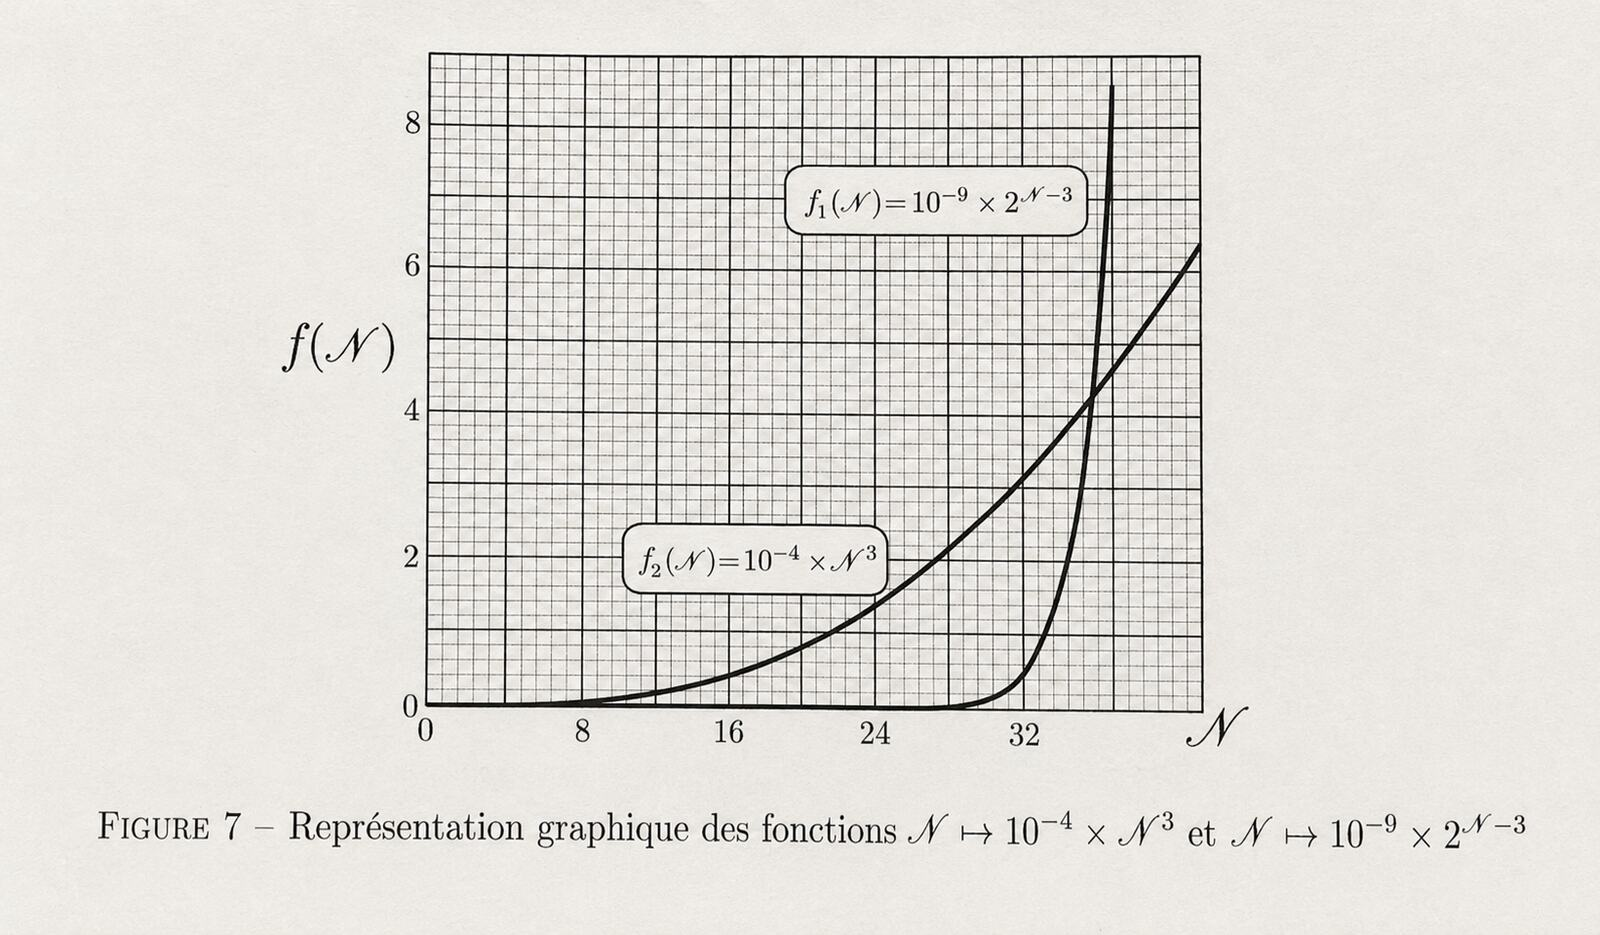
\includegraphics[width=0.72\linewidth]{figure_07.jpg}
\caption{Graphical representation of the functions \(\mathcal{N}\mapsto 10^{-4}\mathcal{N}^{3}\) and \(\mathcal{N}\mapsto 10^{-9}2^{\mathcal{N}-3}\).}
\label{fig:fonctions}
\end{figure}

\end{document}
